% Options for packages loaded elsewhere
% Options for packages loaded elsewhere
\PassOptionsToPackage{unicode}{hyperref}
\PassOptionsToPackage{hyphens}{url}
\PassOptionsToPackage{dvipsnames,svgnames,x11names}{xcolor}
%
\documentclass[
  letterpaper,
  DIV=11,
  numbers=noendperiod,
  sfdefaults=false]{scrartcl}
\usepackage{xcolor}
\usepackage[margin=25mm]{geometry}
\usepackage{amsmath,amssymb}
\setcounter{secnumdepth}{3}
\usepackage{iftex}
\ifPDFTeX
  \usepackage[T1]{fontenc}
  \usepackage[utf8]{inputenc}
  \usepackage{textcomp} % provide euro and other symbols
\else % if luatex or xetex
  \usepackage{unicode-math} % this also loads fontspec
  \defaultfontfeatures{Scale=MatchLowercase}
  \defaultfontfeatures[\rmfamily]{Ligatures=TeX,Scale=1}
\fi
\usepackage{lmodern}
\ifPDFTeX\else
  % xetex/luatex font selection
\fi
% Use upquote if available, for straight quotes in verbatim environments
\IfFileExists{upquote.sty}{\usepackage{upquote}}{}
\IfFileExists{microtype.sty}{% use microtype if available
  \usepackage[]{microtype}
  \UseMicrotypeSet[protrusion]{basicmath} % disable protrusion for tt fonts
}{}
\makeatletter
\@ifundefined{KOMAClassName}{% if non-KOMA class
  \IfFileExists{parskip.sty}{%
    \usepackage{parskip}
  }{% else
    \setlength{\parindent}{0pt}
    \setlength{\parskip}{6pt plus 2pt minus 1pt}}
}{% if KOMA class
  \KOMAoptions{parskip=half}}
\makeatother
% Make \paragraph and \subparagraph free-standing
\makeatletter
\ifx\paragraph\undefined\else
  \let\oldparagraph\paragraph
  \renewcommand{\paragraph}{
    \@ifstar
      \xxxParagraphStar
      \xxxParagraphNoStar
  }
  \newcommand{\xxxParagraphStar}[1]{\oldparagraph*{#1}\mbox{}}
  \newcommand{\xxxParagraphNoStar}[1]{\oldparagraph{#1}\mbox{}}
\fi
\ifx\subparagraph\undefined\else
  \let\oldsubparagraph\subparagraph
  \renewcommand{\subparagraph}{
    \@ifstar
      \xxxSubParagraphStar
      \xxxSubParagraphNoStar
  }
  \newcommand{\xxxSubParagraphStar}[1]{\oldsubparagraph*{#1}\mbox{}}
  \newcommand{\xxxSubParagraphNoStar}[1]{\oldsubparagraph{#1}\mbox{}}
\fi
\makeatother


\usepackage{longtable,booktabs,array}
\newcounter{none} % for unnumbered tables
\usepackage{calc} % for calculating minipage widths
% Correct order of tables after \paragraph or \subparagraph
\usepackage{etoolbox}
\makeatletter
\patchcmd\longtable{\par}{\if@noskipsec\mbox{}\fi\par}{}{}
\makeatother
% Allow footnotes in longtable head/foot
\IfFileExists{footnotehyper.sty}{\usepackage{footnotehyper}}{\usepackage{footnote}}
\makesavenoteenv{longtable}
\usepackage{graphicx}
\makeatletter
\newsavebox\pandoc@box
\newcommand*\pandocbounded[1]{% scales image to fit in text height/width
  \sbox\pandoc@box{#1}%
  \Gscale@div\@tempa{\textheight}{\dimexpr\ht\pandoc@box+\dp\pandoc@box\relax}%
  \Gscale@div\@tempb{\linewidth}{\wd\pandoc@box}%
  \ifdim\@tempb\p@<\@tempa\p@\let\@tempa\@tempb\fi% select the smaller of both
  \ifdim\@tempa\p@<\p@\scalebox{\@tempa}{\usebox\pandoc@box}%
  \else\usebox{\pandoc@box}%
  \fi%
}
% Set default figure placement to htbp
\def\fps@figure{htbp}
\makeatother


% definitions for citeproc citations
\NewDocumentCommand\citeproctext{}{}
\NewDocumentCommand\citeproc{mm}{%
  \begingroup\def\citeproctext{#2}\cite{#1}\endgroup}
\makeatletter
 % allow citations to break across lines
 \let\@cite@ofmt\@firstofone
 % avoid brackets around text for \cite:
 \def\@biblabel#1{}
 \def\@cite#1#2{{#1\if@tempswa , #2\fi}}
\makeatother
\newlength{\cslhangindent}
\setlength{\cslhangindent}{1.5em}
\newlength{\csllabelwidth}
\setlength{\csllabelwidth}{3em}
\newenvironment{CSLReferences}[2] % #1 hanging-indent, #2 entry-spacing
 {\begin{list}{}{%
  \setlength{\itemindent}{0pt}
  \setlength{\leftmargin}{0pt}
  \setlength{\parsep}{0pt}
  % turn on hanging indent if param 1 is 1
  \ifodd #1
   \setlength{\leftmargin}{\cslhangindent}
   \setlength{\itemindent}{-1\cslhangindent}
  \fi
  % set entry spacing
  \setlength{\itemsep}{#2\baselineskip}}}
 {\end{list}}
\usepackage{calc}
\newcommand{\CSLBlock}[1]{\hfill\break\parbox[t]{\linewidth}{\strut\ignorespaces#1\strut}}
\newcommand{\CSLLeftMargin}[1]{\parbox[t]{\csllabelwidth}{\strut#1\strut}}
\newcommand{\CSLRightInline}[1]{\parbox[t]{\linewidth - \csllabelwidth}{\strut#1\strut}}
\newcommand{\CSLIndent}[1]{\hspace{\cslhangindent}#1}



\setlength{\emergencystretch}{3em} % prevent overfull lines

\providecommand{\tightlist}{%
  \setlength{\itemsep}{0pt}\setlength{\parskip}{0pt}}



 


\AtBeginEnvironment{tabular}{\small}
\AtBeginEnvironment{longtable}{\small}
\setkomafont{captionlabel}{\bfseries}
\KOMAoption{captions}{tableheading}
\makeatletter
\@ifpackageloaded{caption}{}{\usepackage{caption}}
\AtBeginDocument{%
\ifdefined\contentsname
  \renewcommand*\contentsname{Table of contents}
\else
  \newcommand\contentsname{Table of contents}
\fi
\ifdefined\listfigurename
  \renewcommand*\listfigurename{List of Figures}
\else
  \newcommand\listfigurename{List of Figures}
\fi
\ifdefined\listtablename
  \renewcommand*\listtablename{List of Tables}
\else
  \newcommand\listtablename{List of Tables}
\fi
\ifdefined\figurename
  \renewcommand*\figurename{Figure}
\else
  \newcommand\figurename{Figure}
\fi
\ifdefined\tablename
  \renewcommand*\tablename{Table}
\else
  \newcommand\tablename{Table}
\fi
}
\@ifpackageloaded{float}{}{\usepackage{float}}
\floatstyle{ruled}
\@ifundefined{c@chapter}{\newfloat{codelisting}{h}{lop}}{\newfloat{codelisting}{h}{lop}[chapter]}
\floatname{codelisting}{Listing}
\newcommand*\listoflistings{\listof{codelisting}{List of Listings}}
\makeatother
\makeatletter
\makeatother
\makeatletter
\@ifpackageloaded{caption}{}{\usepackage{caption}}
\@ifpackageloaded{subcaption}{}{\usepackage{subcaption}}
\makeatother
\usepackage{bookmark}
\IfFileExists{xurl.sty}{\usepackage{xurl}}{} % add URL line breaks if available
\urlstyle{same}
% fallback for those not using the hyperref driver hyperxmp:
\makeatletter
\@ifundefined{xmpquote}{\newcommand{\xmpquote}[1]{#1}}{}
\makeatother
\hypersetup{
  pdftitle={Month 4 methodology: emerging occupation clusters},
  pdfauthor={Antonis Prodromou},
  colorlinks=true,
  linkcolor={blue},
  filecolor={Maroon},
  citecolor={Blue},
  urlcolor={Blue},
  pdfcreator={LaTeX via pandoc}}


\title{Month 4 methodology: emerging occupation clusters}
\author{Antonis Prodromou}
\date{2026-11-25}
\begin{document}
\maketitle


\section{Month 4 methodology: emerging occupation
clusters}\label{month-4-methodology-emerging-occupation-clusters}

This part of the project aims to detectig emerging occupations via
clustering, using the dataset defined in the previous parts, and more
specifically:

\begin{enumerate}
\def\labelenumi{(\alph{enumi})}
\tightlist
\item
  We use the titles of the postings retrieved from the Skillab API and
  we create embeddings for each, using multilingual-e5, which is a
  family of open-source text embedding models designed for cross-lingual
  semantic search, information retrieval, and text representation. These
  models are built on the XLM-RoBERTa architecture, while the model
  sized used has 560M parameters and a 1024-dimensional embedding space.
\item
  Create clusters using HDBSCAN, a machine learning clustering algorithm
  that handles clusters of different shapes and densities. We also
  create a two-dimensional visualisation of the occupation clusters to
  check whether the clustering results are reasonable, using Uniform
  Manifold Approximation and Projection (UMAP). As the embeddings have
  1024 dimensions, we use UMAP to represent them in fewer dimensions
  while attempting to preserve their local neighbourhood structure, and
  plot the postings on a scatter plot. We will also use K-means as a
  comparison, to assess whether HDBSCAN is producing useful clusters
  compared with a more traditional clustering algorithm.
\item
  We will then check whether specific occupations related to
  deglobalization belong or form their own clusters, and record their
  development over quarters between 2024 and 2026. Finally, we will
  calculate the Herfindahl Hirschman Index (HHI)\footnote{The HHI
    (Herfindahl--Hirschman index) is a number between 0 and 1 that shows
    how concentrated postings are. For each region (or employer), it
    takes its share of the cluster's postings, squares each share, and
    adds them up. It is near 0 when postings are spread over many
    regions and equals 1 when they all sit in one. For example, if 3
    regions hold 50\%, 30\% and 20\% of a cluster's postings, the HHI is
    0.25 + 0.09 + 0.04 = 0.38; whereas if all postings were in one
    region it would be 1.} per region and cluster, as well as an
  Occupation Emergence Rate per cluster.
\end{enumerate}

\subsection{Data used}\label{data-used}

The data collected in this part of the study covers the periods before
(defined as ``baselines'') and after specific deglobalization policy
events. The analysis of Month 2 (Table~\ref{tbl-job-postings}) showed
that no board had an adequate number of postings prior to 2024, to be
used for analysis, :

\begin{longtable}[]{@{}
  >{\raggedright\arraybackslash}p{(\linewidth - 14\tabcolsep) * \real{0.0968}}
  >{\raggedleft\arraybackslash}p{(\linewidth - 14\tabcolsep) * \real{0.1290}}
  >{\raggedleft\arraybackslash}p{(\linewidth - 14\tabcolsep) * \real{0.1290}}
  >{\raggedleft\arraybackslash}p{(\linewidth - 14\tabcolsep) * \real{0.1290}}
  >{\raggedleft\arraybackslash}p{(\linewidth - 14\tabcolsep) * \real{0.1290}}
  >{\raggedleft\arraybackslash}p{(\linewidth - 14\tabcolsep) * \real{0.1290}}
  >{\raggedleft\arraybackslash}p{(\linewidth - 14\tabcolsep) * \real{0.1290}}
  >{\raggedleft\arraybackslash}p{(\linewidth - 14\tabcolsep) * \real{0.1290}}@{}}
\caption{Monthly job posting counts across
platforms.}\label{tbl-job-postings}\tabularnewline
\toprule\noalign{}
\begin{minipage}[b]{\linewidth}\raggedright
Month
\end{minipage} & \begin{minipage}[b]{\linewidth}\raggedleft
\texttt{eures}
\end{minipage} & \begin{minipage}[b]{\linewidth}\raggedleft
\texttt{eures-esco}
\end{minipage} & \begin{minipage}[b]{\linewidth}\raggedleft
\texttt{kariera.gr} (GR)
\end{minipage} & \begin{minipage}[b]{\linewidth}\raggedleft
\texttt{lesjeudis.com} (FR)
\end{minipage} & \begin{minipage}[b]{\linewidth}\raggedleft
\texttt{jobbland.se} (SE)
\end{minipage} & \begin{minipage}[b]{\linewidth}\raggedleft
\texttt{jobs.de} (DE)
\end{minipage} & \begin{minipage}[b]{\linewidth}\raggedleft
\texttt{kariera.fr} (FR)
\end{minipage} \\
\midrule\noalign{}
\endfirsthead
\toprule\noalign{}
\begin{minipage}[b]{\linewidth}\raggedright
Month
\end{minipage} & \begin{minipage}[b]{\linewidth}\raggedleft
\texttt{eures}
\end{minipage} & \begin{minipage}[b]{\linewidth}\raggedleft
\texttt{eures-esco}
\end{minipage} & \begin{minipage}[b]{\linewidth}\raggedleft
\texttt{kariera.gr} (GR)
\end{minipage} & \begin{minipage}[b]{\linewidth}\raggedleft
\texttt{lesjeudis.com} (FR)
\end{minipage} & \begin{minipage}[b]{\linewidth}\raggedleft
\texttt{jobbland.se} (SE)
\end{minipage} & \begin{minipage}[b]{\linewidth}\raggedleft
\texttt{jobs.de} (DE)
\end{minipage} & \begin{minipage}[b]{\linewidth}\raggedleft
\texttt{kariera.fr} (FR)
\end{minipage} \\
\midrule\noalign{}
\endhead
\bottomrule\noalign{}
\endlastfoot
2024-01 & 1 & 0 & 0 & 0 & 191 & 0 & 0 \\
2024-02 & 0 & 1 & 0 & 0 & 246 & 0 & 0 \\
2024-03 & 22 & 24 & 0 & 0 & 292 & 0 & 0 \\
2024-04 & 2 & 1 & 0 & 0 & 410 & 0 & 0 \\
2024-05 & 36 & 22 & 0 & 0 & 2,116 & 0 & 0 \\
2024-06 & 3 & 4 & 0 & 0 & 2,879 & 0 & 0 \\
2024-07 & 7 & 2 & 0 & 0 & 2,060 & 0 & 0 \\
2024-08 & 4 & 6 & 2,738 & 5,660 & 4,184 & 3,427 & 3,000 \\
2024-09 & 6 & 5 & 5,629 & 6,649 & 10,034 & 5,632 & 27,099 \\
2024-10 & 5 & 6 & 5,480 & 4,935 & 48,018 & 8,175 & 32,892 \\
2024-11 & 13 & 17 & 5,593 & 3,986 & 50,097 & 6,417 & 7,043 \\
2024-12 & 37 & 62 & 4,866 & 3,511 & 47,151 & 4,029 & 4,941 \\
2025-01 & 270 & 495 & 7,065 & 4,191 & 53,139 & 1,690 & 6,054 \\
2025-02 & 20 & 18 & 3,174 & 1,548 & 23,017 & 2,572 & 4,916 \\
2025-03 & 96 & 62 & 2,884 & 450 & 10,959 & 1,691 & 523 \\
2025-04 & 120 & 93 & 1,458 & 581 & 4,139 & 597 & 0 \\
2025-05 & 91 & 91 & 4,219 & 2,336 & 6,210 & 0 & 0 \\
2025-06 & 64 & 78 & 4,678 & 3,887 & 132 & 0 & 0 \\
2025-07 & 81 & 130 & 4,097 & 800 & 460 & 0 & 0 \\
2025-08 & 148 & 234 & 3,510 & 3,383 & 3,066 & 0 & 0 \\
2025-09 & 937 & 1,610 & 1,703 & 3,279 & 3,968 & 0 & 0 \\
2025-10 & 1,523 & 6,335 & 61 & 1,476 & 1,520 & 0 & 0 \\
2025-11 & 15,811 & 23,611 & 37 & 738 & 3,618 & 0 & 0 \\
2025-12 & 21,926 & 29,746 & 3,308 & 386 & 28,639 & 0 & 0 \\
2026-01 & 99,039 & 130,320 & 7,112 & 250 & 48,511 & 0 & 0 \\
2026-02 & 260,792 & 698,166 & 6,542 & 6,561 & 55,457 & 0 & 0 \\
2026-03 & 0 & 0 & 6,953 & 768 & 62,392 & 0 & 0 \\
2026-04 & 0 & 0 & 6,659 & 0 & 47,721 & 0 & 0 \\
2026-05 & 0 & 0 & 0 & 0 & 53,794 & 0 & 0 \\
2026-06 & 0 & 0 & 0 & 0 & 46,127 & 0 & 0 \\
2026-07 & 0 & 0 & 0 & 0 & 31,166 & 0 & 0 \\
2026-08 & 0 & 0 & 0 & 0 & 40,875 & 0 & 0 \\
2026-09 & 0 & 0 & 0 & 0 & 595 & 0 & 0 \\
\end{longtable}

Our work therefore focuses on two events, using two of these boards:
AccelerateEU (22 April 2026) on jobbland.se and InvestAI (11 February
2025) on lesjeudis.com. It is important to note that the postings of the
individual boards are examined separately and are not merged.

\subsection{Clustering Algorithm Selection and Hyperparameter
Tuning}\label{clustering-algorithm-selection-and-hyperparameter-tuning}

The clustering methodology was developed in two stages:

\begin{enumerate}
\def\labelenumi{\arabic{enumi}.}
\tightlist
\item
  We first compared clustering algorithms and input representations, to
  identify an appropriate approach for grouping job postings.
\item
  Based on the results (see below) HDBSCAN was selected. We then
  conducted a sensitivity analysis to determine the HDBSCAN
  hyperparameter values that lead to the best clusters, i.e.~a
  clustering configuration that produces coherent and interpretable
  groups of job postings, while avoiding too narrow definitions, as well
  as the exclusion of a large proportion of observations.
\end{enumerate}

\paragraph{Generation of Title
Embeddings}\label{generation-of-title-embeddings}

The initial title representations were generated using the pretrained
multilingual-e5-large model (\texttt{intfloat/multilingual-e5-large}).
The model produces a 1,024-dimensional vector for each input text; this
dimensionality is the model's output size, and it was used in its
pretrained form.

The first stage of the process was to clean the job titles using a
python script (script 90). This process removed employer names, location
information, gender markers (such as \texttt{(m/w/d)}) and any job
reference codes. The resulting cleaned titles (\texttt{title\_clean})
were stored for each board in
\texttt{data/tagged/titles\_\textless{}board\textgreater{}.jsonl}. Each
cleaned title was then used as the embedding input (\texttt{text\_a})
(script 92). Where a posting had no title, a title was inferred from the
description, using the Qwen 2.5 7B model (script 99). A human annotator
(i.e.~the author) checked a sample, and it was found that 88\% of the
inferred titles named the same occupation as the real title, which was
deemed satisfactory. The prefix \texttt{query:} was added to each input,
as required by the model's input convention.

\subparagraph{Input representation
encoding}\label{input-representation-encoding}

The text was then encoded using SentenceTransformers, which is a Python
framework built on PyTorch and Transformers for generating embeddings
and computing similarity scores across text. The resulting embeddings
were normalised using L2 normalization (setting
normalize\_embeddings=True), which scales a vector so its Euclidean norm
(length) equals 1 while preserving its direction. This is because
multilingual-e5 is trained so that similar texts point in the same
direction, while the magnitude (length) of each vector is not used in
the comparison. Therefore, by normalising each vector to length 1,
differences in length are removed and the dot product of two titles is
equal to the cosine of the angle between two vectors (``cosine
similarity''). The embeddings were generated using Google Colab, on a T4
GPU. The resulting vectors were saved as NumPy arrays
(\texttt{emb\_\textless{}board\textgreater{}.npy}), with one row per
posting.

Two different UMAP transformations were applied to the 1,024-dimension
title embeddings, serving different purposes:

\begin{enumerate}
\def\labelenumi{(\alph{enumi})}
\tightlist
\item
  In the clustering pipeline (script 92), UMAP reduced the embeddings to
  10 dimensions, using cosine distance, n\_neighbors = 30 and min\_dist
  = 0. The reduction to ten dimensions took place in order to make
  clustering on the basis of density more effective than applying the
  clustering algorithms that followed directly to the original
  1,024-dimensional embeddings; setting min\_dist = 0 allows UMAP to
  place similar observations more closely together, which can make it
  easier for HDBSCAN to identify dense areas.
\item
  At a later stage, for visualisation only, a separate two-dimensional
  UMAP was applied to the original 1,024-dimensional title embeddings.
  The grey points are a random sample of the board's postings, and the
  coloured points are the postings of the clusters selected for
  illustration. Their cluster labels come from the clustering in the
  ten-dimensional UMAP space (script 92) and are only copied onto the
  map. As a reference, the postings whose cleaned title matches the
  pattern of one of the seven occupations listed indicatively in the
  brief are displayed, but these occupations are not used to select or
  form clusters. In other words, this map is a different, indicative
  projection of the original embeddings for visualization purposes,
  therefore the distance between two clusters on the map is not evidence
  of how close they are in the ten-dimensional clustering space.
\end{enumerate}

\paragraph{Comparison of input
representations}\label{comparison-of-input-representations}

Using HDBSCAN as the clustering algorithm (on the aforementioned
10-dimensional UMAP of the embeddings), we examined two input
representations:

\begin{enumerate}
\def\labelenumi{\arabic{enumi}.}
\tightlist
\item
  Input A uses only the cleaned job title, embedded with
  multilingual-e5-large (1,024 dimensions, L2-normalised).
\item
  Input D joins two additional numerical embedding vectors to the title
  embedding via concatenation:

  \begin{enumerate}
  \def\labelenumii{\alph{enumii}.}
  \tightlist
  \item
    An embedding (100 dimensions) of ESCO skills extracted with the
    ESCOX extraction tool (Kavargyris et al. 2025), using a similarity
    threshold of 0.6.
  \item
    An embedding (20 dimensions) of 135 Lightcast terms.
  \end{enumerate}
\end{enumerate}

Input D is further distinguished in two versions:

\begin{enumerate}
\def\labelenumi{\arabic{enumi}.}
\tightlist
\item
  Dv2 uses weights of 0.50 for both ESCOX and Lightcast.
\item
  Dv3 uses weights 0.25 and 0.25 and, in addition, removes very common
  skills before the concatenation. The reason is that our initial runs
  of the concatenated embeddings (that included skills) showed that
  clusters were formed around single skills which were often generic
  (such as ``assume responsibility'', ``meet commitments'',
  ``communicate with customers'' or language skills). These generic
  skills reveal little about the actual role, but still result to
  joining those postings in the same clusters. To remove common skills,
  we followed the following steps:
\end{enumerate}

\subparagraph{Removing generic skills
(Dv3)}\label{removing-generic-skills-dv3}

\textbf{Step 1.} For each board, we count the share of its postings in
which each ESCO skill appears (script 92 and 125).
Table~\ref{tbl-esco-skills} shows an example of ESCO skills for the
lesjeudis board (18,625 postings). The share provided is the number of
postings with the skill divided by all postings of the board, including
postings without any skill; while the skill names are shortened for
clarity (e.g.~``innovation processes The techniques, mod\ldots{}'' is
given below as ``innovation processes'').

\begin{longtable}[]{@{}lrr@{}}
\caption{Selected ESCO skills and their posting
shares}\label{tbl-esco-skills}\tabularnewline
\toprule\noalign{}
ESCO skill & Postings & Share \\
\midrule\noalign{}
\endfirsthead
\toprule\noalign{}
ESCO skill & Postings & Share \\
\midrule\noalign{}
\endhead
\bottomrule\noalign{}
\endlastfoot
innovation processes & 2,412 & 13.0\% \\
cyber security & 2,239 & 12.0\% \\
DevOps & 1,621 & 8.70\% \\
quantum mechanics & 914 & 4.91\% \\
provide user documentation & 899 & 4.83\% \\
\end{longtable}

\textbf{Step 2.} To identify which skills have unusually high
occurrence, and therefore have limited discriminatory value for
distinguishing job roles, we need to examine their distribution. One
approach is to (a) calculate the share of postings in which each item
appears (b) rank the items (skills or terms) by that share and (c)
remove the outliers, which in this case are the most common terms.

Plotting the distribution of skill occurrence, it was found to be
right-skewed: most skills (inliers) appeared in relatively few postings,
while only a small number (outliers) appeared in many of them. To
account for this skewness, we applied a logarithmic transformation to
the shares and then used the Tukey boxplot rule (Tukey 1977) to identify
the boundary between inliers and outliers. According to this, a skill is
considered unusually frequent if its log share exceeds the upper fence,
calculated as Q3 + 1.5 × IQR, where Q3 and IQR are calculated from the
distribution of log-transformed shares.

The fence was estimated at 4.9\% for the lesjeudis board, 1.5\% for
jobs.de and 1.6\% for jobbland. The result was that it removed 26, 31
and 56 skills, respectively.

\begin{figure}

\centering{

\pandocbounded{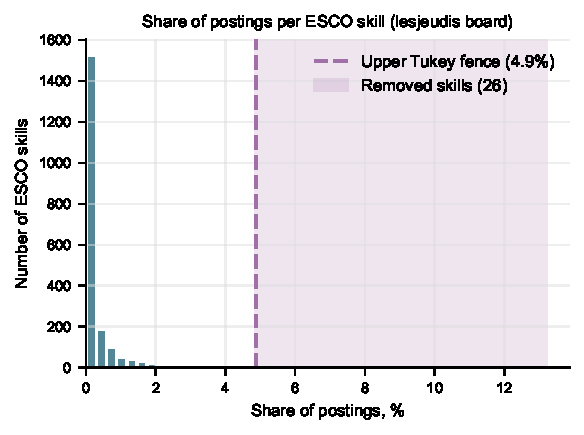
\includegraphics[keepaspectratio]{Month_4_methodology_akp_files/figure-pdf/fig-tukey-output-1.pdf}}

}

\caption{\label{fig-tukey}Share of postings per ESCO skill on lesjeudis.
The dashed line is the upper Tukey fence (4.9\%); the 26 skills above it
are removed in Dv3.}

\end{figure}%

It should be noted that the Lightcast terms were not found to exceed the
upper Tuckey threshold (the largest share is 4.8\%, for ``Supply Chain''
on the lesjeudis board), so the Tukey fence was applied to ESCO skills
only.

\textbf{Step 3.} We next wanted to keep the most useful skills, in the
sense of determining which ones are associated with particular types of
jobs, but removing skills that appear in very different types of jobs.
Similarly to Step 2, this approach also aims to remove generic skills,
but this time by examining their variance rather than their frequency
alone. For example, the skill ``communication'' might appear across many
different job types, whereas ``Machine learning'' might appear
frequently within data analysis jobs but rarely elsewhere. It is
therefore more useful for distinguishing those jobs.

For this purpose, we use the similarity between job titles as an
indication of how closely related two postings are, represented through
a k-nearest-neighbour (k-NN) graph. The graph forms a network of job
postings in which each posting is connected to its (k) most similar
postings, based on their title embeddings. We set (k=5), meaning that
each posting considers its five most similar neighbours. We consider
that in this case a smaller neighbourhood (lower k) makes sense because
we want to assess how closely a skill is associated with the most
similar job titles, rather than with a broader set of jobs. A link is
considered to exist if either posting is among the other's neighbours.

To evaluate whether a skill tends to appear in similar job postings, we
decided to use the Laplacian Score (He et al. 2005). This is an
unsupervised feature-selection method that scores each feature by how
well its values agree with a neighbourhood graph of the samples. In our
case the samples are the job postings, and each skill is a feature,
which is assigned 1 for the postings tagged with the skill and 0 for all
others. We chose the method because we have no occupation labels, so an
unsupervised method is needed, and because it checks, for each skill,
whether the postings tagged with it are close to each other in the title
embedding space, i.e.~whether they are neighbours in the graph, and
therefore semantically related.

As part of this technique, for every skill and term, we score how well
the set of postings that include it follow this graph. The score is low
if the postings that carry the item are neighbours and close to 1 if the
item is unrelated to the graph. The calculation involves the following
steps:

\begin{enumerate}
\def\labelenumi{(\alph{enumi})}
\item
  For each skill, we create a vector of n size, where n is the number of
  postings in the graph. The vector components are assigned 1 when a
  posting contains the skill and 0 when it does not.
\item
  For each link connecting the postings in the graph, we calculate its
  weight, which is equal to:
\end{enumerate}

\[
w_{ij} = \exp\left(-\frac{d_{ij}^{2}}{t}\right)
\]

where:

\begin{itemize}
\tightlist
\item
  (d\_\{ij\}) is the distance between the title embeddings of postings
  (i) and (j).
\end{itemize}

Since the embeddings are unit-length vectors, cosine distance can be
calculated as:

\[
d_{ij} = 1 - \cos(\theta_{ij})
\]

where (\cos(\theta\_\{ij\})) is the cosine similarity between the two
job-title embeddings, with similar titles having a close distance.

\begin{itemize}
\tightlist
\item
  \begin{enumerate}
  \def\labelenumi{(\alph{enumi})}
  \setcounter{enumi}{19}
  \tightlist
  \item
    is the kernel bandwidth, whuch controls how quickly the link weight
    decreases as the distance between titles increases, and is defined
    as:
  \end{enumerate}
\end{itemize}

\[
t = \text{mean squared distance over links between different titles}
\]

\begin{enumerate}
\def\labelenumi{(\alph{enumi})}
\setcounter{enumi}{2}
\tightlist
\item
  We calculate the weighted mean of each skill and center the skill
  vector by extracting it from the original 0 and 1 values: {[}
  z\_i=x\_i-\bar\{x\}\_w {]}
\end{enumerate}

This results to postings carrying the skill being positing and postings
not carrying it negative.

\begin{enumerate}
\def\labelenumi{(\alph{enumi})}
\setcounter{enumi}{3}
\tightlist
\item
  We finally calculate the Laplacian score, equal to:
\end{enumerate}

\[
S = \frac{N}{D}
\]

where:

\begin{itemize}
\tightlist
\item
  The numerator is the weighted differences in skill values across graph
  links:
\end{itemize}

\[
N = \sum_{(i,j)\in E} w_{ij}(x_i-x_j)^2
\]

where:

\begin{itemize}
\item
  (E) is the set of graph links.
\item
  (w\_\{ij\}) is the weight of the link between postings (i) and (j).
\item
  (x\_i) and (x\_j) are the binary skill indicators (0 or 1) for
  postings (i) and (j), respectively.
\item
  The denominator is the overall weighted variation in skill values
  across all postings:
\end{itemize}

\[
D = \sum_i d_i(x_i-\bar{x}_w)^2
\]

where:

\begin{itemize}
\tightlist
\item
  (d\_i) is the weighted degree of posting (i), calculated as the sum of
  the weights of its connected links.
\item
  (x\_i) is the binary skill indicator for posting (i).
\item
  (\bar\{x\}\_w) is the weighted mean of the skill indicators across all
  postings.
\end{itemize}

A lower score indicates that postings containing the skill tend to be
connected to other postings containing the same skill. A higher score
indicates that the skill is more dispersed across the title-based graph.

In the below example, assuming that in the k-NN graph (a) Data
Scientist, Data Analyst and ML Engineer are closely connected and (b) HR
Manager, Recruiter and HR Assistant are also closely connected, the
``communication'' skill appears in two technology-related postings, as
well as two HR-related postings; as its occurrence is spread across
different types of jobs, it is less closely aligned with the graph
structure and we would expect it to receive a higher Laplacian Score
than e.g.~``Python'', which appears only in technology-related postings.

\textbf{Table: Example of job postings (samples) and skills (features)}

\begin{longtable}[]{@{}lrrr@{}}
\caption{Binary representation of skills across job
postings}\label{tbl-sample-features}\tabularnewline
\toprule\noalign{}
Sample (job posting) & Python & Data analysis & Communication \\
\midrule\noalign{}
\endfirsthead
\toprule\noalign{}
Sample (job posting) & Python & Data analysis & Communication \\
\midrule\noalign{}
\endhead
\bottomrule\noalign{}
\endlastfoot
Data Scientist & 1 & 1 & 1 \\
Data Analyst & 1 & 1 & 1 \\
ML Engineer & 1 & 0 & 0 \\
HR Manager & 0 & 0 & 1 \\
Recruiter & 0 & 0 & 1 \\
HR Assistant & 0 & 0 & 0 \\
\end{longtable}

However, it is important to note that the Laplacian Score cannot remove
false matches that are consistent. For example, we found that it kept
``feed concrete mixer'' (score 0.301), despite it being linked to
irrelevant job titles between them. The explanation might be that this
skill is about supplying a machine with the right materials. A sentence
in a job advert, such as ``supply the client with\ldots'', ``provide the
necessary\ldots'' or ``ensure delivery of\ldots'', can be similar enough
in meaning to cross the 0.6 threshold of the ESCOX algorithm.

\textbf{Step 4.} The orignal Laplacian Score paper ranks the features
rather than applying a cut-off, so in order to follow it, we compared
the clustering for thresholds 0.7, 0.8, 0.9 and 1.0 on lesjeudis
(silhouette, noise, seed stability). The threshold 1.0 keeps 99\% of the
items, because an item unrelated to the graph scores about 1. The
threshold 0.8 gave the lowest noise and the highest silhouette in the
UMAP space for Dv2, and it was therefore decided to be used for both
versions and all boards. This keeps 204 (Dv2) and 190 (Dv3) of the ESCO
skills on lesjeudis, 130 and 114 on jobs.de, and 205 and 198 on
jobbland. Regarding Lightcast, it kept 4 terms on lesjeudis, none on
jobs.de and one on jobbland.

The tables in Section~\ref{sec-appendix-ls} show, for jobbland, the 15
skills with the lowest and the 15 with the highest score. The lowest
scores belong mostly to skills with few postings whose postings carry
similar titles, for example mystery shopping or babysitting. The highest
scores (1.000 to 1.001) belong to skills whose postings are spread over
unrelated titles, including specific healthcare skills such as medical
laboratory technology. The score measures whether the postings of a
skill are concentrated among similar titles, not whether the skill was
assigned correctly. A wrongly assigned skill whose postings happen to
share similar titles also scores low (for example ``improve chemical
processes'', whose most common title is ``junior audit consultants''),
and a correct skill used across many different roles is dropped. We
therefore use the score as a filter for skills that are concentrated
among similar titles, and not as a check of the skill tagging itself.
The frequency cut and the score also act on different skills: ``give
interviews to media'' (1,379 postings) is kept by the score but removed
by the Tukey cut in Dv3.

\textbf{Step 5.} The remaining skills / terms were finally weighted with
TF-IDF and reduced with TruncatedSVD, to 100 dimensions for ESCO and 20
for Lightcast. Each block was normalised to unit length, multiplied by
its weight, concatenated with the title embedding (weight 1) and
normalised again. A posting that loses all its items gets zeros in the
skill embeddings, so it is clustered on its title alone.

\subparagraph{Results}\label{results}

We compared the three input cariations on lesjeudis.com with two
criteria from the literature on text clustering with embeddings. The
first is the silhouette (Rousseeuw 1987), computed in the space in which
each input was clustered (the 10-dimensional UMAP space) and in the
original embedding space. In simple terms, the silhouette measures how
compact the clusters are in the space they take up.

The second is topic coherence (C\textsubscript{NPMI}), a standard
semantic measure used for clusters of text (Röder et al. 2015;
Grootendorst 2022). For each cluster we took the ten words with the
highest class-based tf-idf score in its titles (Grootendorst 2022) and
computed the mean normalised pointwise mutual information (Bouma 2009)
over all pairs of these words. Each title of the board counts as one
document. C\textsubscript{NPMI} is −1 when two words never occur in the
same title and +1 when they always do.

{\def\LTcaptype{none} % do not increment counter
\begin{longtable}[]{@{}
  >{\raggedright\arraybackslash}p{(\linewidth - 10\tabcolsep) * \real{0.1667}}
  >{\raggedright\arraybackslash}p{(\linewidth - 10\tabcolsep) * \real{0.1667}}
  >{\raggedright\arraybackslash}p{(\linewidth - 10\tabcolsep) * \real{0.1667}}
  >{\raggedright\arraybackslash}p{(\linewidth - 10\tabcolsep) * \real{0.1667}}
  >{\raggedright\arraybackslash}p{(\linewidth - 10\tabcolsep) * \real{0.1667}}
  >{\raggedright\arraybackslash}p{(\linewidth - 10\tabcolsep) * \real{0.1667}}@{}}
\toprule\noalign{}
\begin{minipage}[b]{\linewidth}\raggedright
Input
\end{minipage} & \begin{minipage}[b]{\linewidth}\raggedright
Clusters
\end{minipage} & \begin{minipage}[b]{\linewidth}\raggedright
Noise
\end{minipage} & \begin{minipage}[b]{\linewidth}\raggedright
Silhouette, UMAP space / input space
\end{minipage} & \begin{minipage}[b]{\linewidth}\raggedright
Median C\textsubscript{NPMI}
\end{minipage} & \begin{minipage}[b]{\linewidth}\raggedright
Mean C\textsubscript{NPMI}, weighted by postings
\end{minipage} \\
\midrule\noalign{}
\endhead
\bottomrule\noalign{}
\endlastfoot
A & 144 & 30.9\% & 0.618 / 0.087 & −0.389 & −0.342 \\
D v2 & 142 & 20.6\% & 0.735 / 0.170 & −0.485 & −0.447 \\
D v3 & 102 & 30.6\% & 0.590 / 0.090 & −0.376 & −0.273 \\
\end{longtable}
}

According to the silhouette score, input D v2 is the preferred choice
(0.735 against 0.618 for A, in the UMAP space), and it also has the
least noise. In input D, however, the clustering space includes the ESCO
skills and Lightcast terms, so postings can be closer in the embedding
space not because their titles are similar but because of their skills.

It is therefore expected that topic coherence (C\textsubscript{NPMI}),
which looks only at the words of the titles, gives the opposite result:
D v2 has the lowest values (median C\textsubscript{NPMI} −0.485 against
−0.389 for A), which means that the titles inside its clusters share
fewer words than those of A. The reason is that skills can be unreliable
because of how they are extracted. The esco-skill-extractor turns each
piece of a posting into a vector with a small sentence model
(all-MiniLM-L6-v2) and compares it with the vector of every ESCO skill
description. A skill counts as found when the similarity reaches 0.6. In
the first version of input D (D v1), which had no coherence filter, this
produced false matches such as the skill ``feed concrete mixer'' on IT
consultants' postings. This can be due to (a) generic wording, because a
common sentence of a job advert such as ``supply the client
with\ldots{}'' or ``ensure delivery of\ldots{}'' can be similar in
meaning in the context of a skill description or (b) employer templates,
because one sentence repeated in a group of postings, such as a company
description, gives the same skill to all of them. The coherence filter
in D v2 and D v3 was introduced to remove skills whose postings have
unrelated titles.

Input D v3 is similar to A on both criteria (silhouette 0.590 against
0.618; median C\textsubscript{NPMI} −0.376 against −0.389; weighted mean
−0.273 against −0.342) but xxxx. We therefore keep input A as the main
input and D v3 as a sensitivity check.

C\textsubscript{NPMI} is negative for all three inputs. This can be
explained by the fact that titles are very short documents, and the top
words of a cluster are mostly alternative words for the same role (for
example ``buyer'' and ``purchasing'') or rare tokens which rarely occur
in the same title. In the lesjeudis board, about one fifth of the titles
(at least 21.7\%) contain French, so some of the top words are French
equivalents of English ones (for example ``buyer'' and ``acheteur'').
The values are therefore compared with each other and not interpreted in
absolute terms. The silhouette comes from the algorithm comparison, and
C\textsubscript{NPMI} from the saved cluster labels of a separate run of
the same settings, so the numbers of clusters and noise differ slightly
between the two (for example 136 and 142 clusters for D v2).

\paragraph{Clustering algorithms
tested}\label{clustering-algorithms-tested}

Using the embeddings of Case A (i.e.~ectracted only from the title) as
input, we next compared the results of four clustering algorithms on the
postings: 1. HDBSCAN with excess-of-mass (EOM) cluster selection 2.
HDBSCAN with leaf cluster selection 3. k-means 4. Ward agglomerative
clustering.

All methods were applied to the same 10-dimensional UMAP representations
of the input embeddings, so that the results can be compared on the same
dimensional space. The number of clusters was set to XXX for all
algorithms, because xxxx. This provided a comparison between the methods
the a similar level of cluster granularity. For the k-means algorithm in
specific, we also examined five alternative values of k (25, 50, 100,
200 and 400) to investigate how the number of clusters affected the
resulting silhouette scores.

The comparison was conducted on the three job-posting platforms that had
already been chosen due to their data completeness over time (LesJeudis,
Jobbland and Jobs.de).

\subparagraph{Evaluation criteria}\label{evaluation-criteria}

Clustering quality was assessed using the silhouette coefficient,
calculated on a random sample of 10,000 postings (random seed 1). The
silhouette coefficient measures how well an observation fits within its
assigned cluster relative to the nearest alternative cluster. It ranges
from -1 to +1, with higher values indicating better-defined cluster
assignments.

For an individual observation, the silhouette coefficient is calculated
as:

\[
s(i) = \frac{b(i)-a(i)}{\max(a(i),b(i))}
\]

where \(a(i)\) represents the average distance between observation \(i\)
and the other observations in its assigned cluster, and \(b(i)\)
represents the lowest average distance between observation \(i\) and the
observations in another cluster (i.e.~the nearest alternative cluster).

Silhouette scores were calculated in two spaces: the 10-dimensional UMAP
space, using Euclidean distance, and the original embedding space, using
cosine distance. This provided two complementary assessments: the
separation of clusters in the space used for clustering and the
separation of the same cluster assignments in the original embedding
space.

Since HDBSCAN can leave observations unassigned, the proportion of
postings classified as noise was reported alongside its silhouette
scores. This was important because the silhouette is calculated only for
observations assigned to clusters, meaning that an algorithm could
obtain a relatively high score by excluding difficult-to-cluster
postings. To address this issue further, k-means and Ward were also
evaluated on the subset of postings assigned to clusters by HDBSCAN EOM,
allowing their silhouette scores to be compared on the same
observations.

\paragraph{HDBSCAN EOM and leaf
selection}\label{hdbscan-eom-and-leaf-selection}

Table 1 reports the number of clusters, noise proportion and silhouette
scores obtained using HDBSCAN EOM and leaf selection across the three
datasets and input representations.

\textbf{Table 1. HDBSCAN EOM and leaf comparison across datasets and
input representations}

{\def\LTcaptype{none} % do not increment counter
\begin{longtable}[]{@{}
  >{\raggedright\arraybackslash}p{(\linewidth - 14\tabcolsep) * \real{0.1250}}
  >{\raggedright\arraybackslash}p{(\linewidth - 14\tabcolsep) * \real{0.1250}}
  >{\raggedleft\arraybackslash}p{(\linewidth - 14\tabcolsep) * \real{0.1250}}
  >{\raggedleft\arraybackslash}p{(\linewidth - 14\tabcolsep) * \real{0.1250}}
  >{\raggedleft\arraybackslash}p{(\linewidth - 14\tabcolsep) * \real{0.1250}}
  >{\raggedleft\arraybackslash}p{(\linewidth - 14\tabcolsep) * \real{0.1250}}
  >{\raggedleft\arraybackslash}p{(\linewidth - 14\tabcolsep) * \real{0.1250}}
  >{\raggedleft\arraybackslash}p{(\linewidth - 14\tabcolsep) * \real{0.1250}}@{}}
\toprule\noalign{}
\begin{minipage}[b]{\linewidth}\raggedright
Dataset
\end{minipage} & \begin{minipage}[b]{\linewidth}\raggedright
Input
\end{minipage} & \begin{minipage}[b]{\linewidth}\raggedleft
EOM clusters
\end{minipage} & \begin{minipage}[b]{\linewidth}\raggedleft
EOM noise (\%)
\end{minipage} & \begin{minipage}[b]{\linewidth}\raggedleft
EOM silhouette (UMAP)
\end{minipage} & \begin{minipage}[b]{\linewidth}\raggedleft
EOM silhouette (input)
\end{minipage} & \begin{minipage}[b]{\linewidth}\raggedleft
Leaf clusters
\end{minipage} & \begin{minipage}[b]{\linewidth}\raggedleft
Leaf noise (\%)
\end{minipage} \\
\midrule\noalign{}
\endhead
\bottomrule\noalign{}
\endlastfoot
LesJeudis & A & 144 & 30.9 & 0.618 & 0.087 & 151 & 32.5 \\
LesJeudis & D & 136 & 21.1 & 0.735 & 0.170 & 148 & 26.5 \\
Jobbland & A & 357 & 34.3 & 0.618 & 0.071 & 391 & 40.3 \\
Jobbland & D & 263 & 20.2 & 0.707 & 0.122 & 290 & 29.1 \\
Jobs.de & A & 71 & 27.6 & 0.542 & 0.086 & 84 & 38.8 \\
Jobs.de & D & 102 & 25.2 & 0.711 & 0.163 & 109 & 28.9 \\
LesJeudis & D v3 & 101 & 29.8 & 0.590 & 0.090 & 121 & 38.6 \\
Jobbland & D v3 & 282 & 36.3 & 0.627 & 0.098 & 308 & 42.2 \\
Jobs.de & D v3 & 65 & 32.5 & 0.592 & 0.119 & 75 & 40.1 \\
\end{longtable}
}

\emph{Note: Silhouette scores are calculated in the UMAP and original
embedding spaces, respectively. Noise percentages refer to the
proportion of postings not assigned to a cluster.}

The comparison indicated that HDBSCAN generally achieved higher
silhouette scores in the UMAP space than k-means and Ward when the
latter were required to assign every posting to a cluster. However, the
difference became substantially smaller when k-means and Ward were
evaluated only on the postings retained by HDBSCAN EOM. This suggested
that a substantial part of HDBSCAN's advantage resulted from its ability
to identify and exclude observations that did not fit sufficiently well
into dense clusters.

In the original embedding space, silhouette scores were considerably
lower across all methods, with all values below 0.17. The results did
not establish a consistent advantage for any algorithm. This distinction
was important because HDBSCAN identified clusters in the UMAP space,
meaning that silhouette scores calculated in that same space were not an
independent basis for establishing the occupational quality of the
resulting clusters.

The comparison also showed that HDBSCAN leaf selection generally
produced more clusters and a higher proportion of noise than EOM, while
providing only modest improvements in UMAP silhouette scores. Across the
six principal dataset and input combinations, leaf selection produced
between 7 and 34 additional clusters. Its silhouette improvements in
UMAP space were generally limited, while the proportion of noise
increased in several cases. It was therefore retained as an alternative
specification for sensitivity analysis rather than selected as the main
approach.

\paragraph{Comparison of HDBSCAN EOM with k-means and Ward agglomerative
clustering}\label{comparison-of-hdbscan-eom-with-k-means-and-ward-agglomerative-clustering}

Table 2 presents the silhouette scores for k-means and Ward clustering,
using the same number of clusters as HDBSCAN EOM. The final two columns
report the scores obtained when these methods were evaluated only on the
subset of postings assigned to clusters by HDBSCAN EOM.

\textbf{Table 2. Silhouette comparison of k-means and Ward clustering}

{\def\LTcaptype{none} % do not increment counter
\begin{longtable}[]{@{}
  >{\raggedright\arraybackslash}p{(\linewidth - 14\tabcolsep) * \real{0.1250}}
  >{\raggedright\arraybackslash}p{(\linewidth - 14\tabcolsep) * \real{0.1250}}
  >{\raggedleft\arraybackslash}p{(\linewidth - 14\tabcolsep) * \real{0.1250}}
  >{\raggedleft\arraybackslash}p{(\linewidth - 14\tabcolsep) * \real{0.1250}}
  >{\raggedleft\arraybackslash}p{(\linewidth - 14\tabcolsep) * \real{0.1250}}
  >{\raggedleft\arraybackslash}p{(\linewidth - 14\tabcolsep) * \real{0.1250}}
  >{\raggedleft\arraybackslash}p{(\linewidth - 14\tabcolsep) * \real{0.1250}}
  >{\raggedleft\arraybackslash}p{(\linewidth - 14\tabcolsep) * \real{0.1250}}@{}}
\toprule\noalign{}
\begin{minipage}[b]{\linewidth}\raggedright
Dataset
\end{minipage} & \begin{minipage}[b]{\linewidth}\raggedright
Input
\end{minipage} & \begin{minipage}[b]{\linewidth}\raggedleft
k-means (UMAP)
\end{minipage} & \begin{minipage}[b]{\linewidth}\raggedleft
k-means (input)
\end{minipage} & \begin{minipage}[b]{\linewidth}\raggedleft
Ward (UMAP)
\end{minipage} & \begin{minipage}[b]{\linewidth}\raggedleft
Ward (input)
\end{minipage} & \begin{minipage}[b]{\linewidth}\raggedleft
k-means (EOM subset)
\end{minipage} & \begin{minipage}[b]{\linewidth}\raggedleft
Ward (EOM subset)
\end{minipage} \\
\midrule\noalign{}
\endhead
\bottomrule\noalign{}
\endlastfoot
LesJeudis & A & 0.467 & 0.030 & 0.461 & 0.026 & 0.576 & 0.593 \\
LesJeudis & D & 0.615 & 0.118 & 0.609 & 0.115 & 0.720 & 0.716 \\
Jobbland & A & 0.438 & -0.014 & 0.433 & -0.022 & 0.577 & 0.587 \\
Jobbland & D & 0.608 & 0.089 & 0.603 & 0.090 & 0.704 & 0.703 \\
Jobs.de & A & 0.431 & 0.023 & 0.417 & 0.052 & 0.519 & 0.528 \\
Jobs.de & D & 0.539 & 0.088 & 0.537 & 0.081 & 0.638 & 0.646 \\
LesJeudis & D v3 & 0.476 & 0.058 & 0.459 & 0.055 & 0.567 & 0.581 \\
Jobbland & D v3 & 0.433 & 0.028 & 0.417 & 0.024 & 0.595 & 0.603 \\
Jobs.de & D v3 & 0.416 & 0.059 & 0.415 & 0.053 & 0.540 & 0.540 \\
\end{longtable}
}

\emph{Note: The first four silhouette columns report scores in UMAP and
original embedding spaces. The final two columns report scores in UMAP
space, calculated on the subset of postings assigned to clusters by
HDBSCAN EOM.}

The results show that k-means and Ward generally obtained lower UMAP
silhouette scores than HDBSCAN EOM when all postings were required to be
assigned to a cluster. However, when evaluated on the same postings
retained by HDBSCAN, the differences became considerably smaller. For
example, on Jobbland D, the UMAP silhouette scores were 0.707 for
HDBSCAN EOM, 0.704 for k-means and 0.703 for Ward. This demonstrates
that HDBSCAN's ability to leave difficult-to-cluster observations
unassigned is an important factor behind its higher silhouette scores.

In the original embedding space, the scores were generally low, with
k-means and Ward even producing slightly negative values for Jobbland A.
Ward also obtained scores equal to or higher than HDBSCAN EOM on the
EOM-retained postings in three of the six principal dataset and input
combinations. Consequently, the original embedding-space results did not
provide sufficient evidence to establish a clear advantage for HDBSCAN
over the alternative algorithms.

\paragraph{Sensitivity of k-means to the number of
clusters}\label{sensitivity-of-k-means-to-the-number-of-clusters}

A separate k-means experiment examined the effect of different values of
k on the resulting silhouette scores. The five values tested were 25,
50, 100, 200 and 400.

\textbf{Table 3. k-means silhouette scores for alternative numbers of
clusters}

{\def\LTcaptype{none} % do not increment counter
\begin{longtable}[]{@{}llrrrrr@{}}
\toprule\noalign{}
Dataset & Input & k = 25 & k = 50 & k = 100 & k = 200 & k = 400 \\
\midrule\noalign{}
\endhead
\bottomrule\noalign{}
\endlastfoot
LesJeudis & A & 0.358 & 0.389 & 0.426 & 0.495 & 0.526 \\
LesJeudis & D & 0.512 & 0.497 & 0.575 & 0.622 & 0.570 \\
Jobbland & A & 0.384 & 0.400 & 0.384 & 0.420 & 0.441 \\
Jobbland & D & 0.362 & 0.413 & 0.527 & 0.610 & 0.560 \\
Jobs.de & A & 0.404 & 0.404 & 0.434 & 0.473 & 0.497 \\
Jobs.de & D & 0.440 & 0.469 & 0.536 & 0.618 & 0.615 \\
LesJeudis & D v3 & 0.408 & 0.444 & 0.474 & 0.473 & 0.455 \\
Jobbland & D v3 & 0.351 & 0.387 & 0.407 & 0.430 & 0.439 \\
Jobs.de & D v3 & 0.425 & 0.438 & 0.422 & 0.459 & 0.465 \\
\end{longtable}
}

\emph{Note: All silhouette scores are calculated in the 10-dimensional
UMAP space.}

The k-means experiment did not identify a consistent optimal number of
clusters across datasets and input representations. Silhouette scores
generally increased with k in some configurations, while others
exhibited peaks or relatively flat patterns. For input A, the scores
increased with k for LesJeudis and Jobs.de, while Jobbland exhibited a
comparatively flatter pattern. For input D, the scores peaked at k = 200
for all three datasets, although the difference between k = 200 and k =
400 was small for Jobs.de.

Consequently, the results did not provide a clear basis for selecting a
particular number of clusters independently of the clustering algorithm.
The number of clusters produced by HDBSCAN was therefore determined by
its density-based clustering parameters rather than by attempting to
optimise the silhouette through a predetermined value of k.

\subsubsection{Selection of HDBSCAN
Hyperparameters}\label{selection-of-hdbscan-hyperparameters}

Following the selection of HDBSCAN EOM, a second stage examined the
sensitivity of the clustering results to the choice of two
hyperparameters: \texttt{min\_cluster\_size} and \texttt{min\_samples}.

The \texttt{min\_cluster\_size} parameter specifies the minimum number
of observations required for a group to be considered a cluster. The
\texttt{min\_samples} parameter controls the density requirement for
observations to be assigned to a cluster rather than classified as
noise. Increasing \texttt{min\_samples} generally makes the clustering
more conservative, as a higher local density is required for
observations to be considered part of a cluster.

The experiments were conducted using the LesJeudis dataset and input A,
with the same input embeddings and
\texttt{cluster\_selection\_method=\textquotesingle{}eom\textquotesingle{}}
held constant. The initial grid comprised five parameter combinations:
(10, 10), (20, 10), (20, 20), (40, 10) and (40, 40), where the first
value denotes \texttt{min\_cluster\_size} and the second denotes
\texttt{min\_samples}. The grid was subsequently extended to include
(80, 20) and (80, 40), in order to investigate whether larger minimum
cluster sizes could produce fewer, more substantial clusters.

Each configuration was evaluated using two random seeds. The resulting
solutions were compared using several criteria:

\begin{itemize}
\tightlist
\item
  \textbf{Number of clusters:} to assess the overall granularity of the
  clustering and whether the resulting number of groups was manageable
  for subsequent analysis.
\item
  \textbf{Percentage of noise observations:} the proportion of postings
  that HDBSCAN did not assign to any cluster, indicating how restrictive
  the density requirements were.
\item
  \textbf{Median cluster size:} to assess the typical size of the
  resulting clusters.
\item
  \textbf{Number of small clusters:} the number of clusters containing
  fewer than 60 postings, providing an indication of how many relatively
  small groups were produced.
\item
  \textbf{Relative validity:} HDBSCAN's internal density-based validity
  measure, used as an additional indicator of clustering quality.
\item
  \textbf{Agreement between random seeds:} measured using the Adjusted
  Rand Index (ARI), calculated on postings assigned to clusters in both
  runs. An ARI of 1 indicates identical cluster assignments, while lower
  values indicate greater differences.
\item
  \textbf{Named-occupation coverage:} an exploratory check of whether
  four manually identified occupation titles in the LesJeudis dataset
  (three related to export control and one to semiconductor occupations)
  were assigned to clusters rather than classified as noise.
\end{itemize}

The objective was not simply to maximise the number of clusters or
minimise the proportion of noise. Rather, the aim was to identify a
reasonable balance between cluster granularity, cluster size, the
retention of observations, internal clustering quality and
reproducibility. Particular attention was paid to avoiding an excessive
number of small clusters, given the requirements of the subsequent
occupational analysis.

\paragraph{Hyperparameter sensitivity
results}\label{hyperparameter-sensitivity-results}

Table 4 reports the results of the extended hyperparameter grid, using
the second experimental run conducted on 18 November.

\textbf{Table 4. HDBSCAN hyperparameter sensitivity analysis (LesJeudis,
Input A)}

{\def\LTcaptype{none} % do not increment counter
\begin{longtable}[]{@{}
  >{\raggedleft\arraybackslash}p{(\linewidth - 10\tabcolsep) * \real{0.1667}}
  >{\raggedleft\arraybackslash}p{(\linewidth - 10\tabcolsep) * \real{0.1667}}
  >{\raggedleft\arraybackslash}p{(\linewidth - 10\tabcolsep) * \real{0.1667}}
  >{\raggedleft\arraybackslash}p{(\linewidth - 10\tabcolsep) * \real{0.1667}}
  >{\raggedleft\arraybackslash}p{(\linewidth - 10\tabcolsep) * \real{0.1667}}
  >{\raggedleft\arraybackslash}p{(\linewidth - 10\tabcolsep) * \real{0.1667}}@{}}
\toprule\noalign{}
\begin{minipage}[b]{\linewidth}\raggedleft
\texttt{min\_cluster\_size}
\end{minipage} & \begin{minipage}[b]{\linewidth}\raggedleft
\texttt{min\_samples}
\end{minipage} & \begin{minipage}[b]{\linewidth}\raggedleft
Clusters
\end{minipage} & \begin{minipage}[b]{\linewidth}\raggedleft
Noise (\%)
\end{minipage} & \begin{minipage}[b]{\linewidth}\raggedleft
Median size
\end{minipage} & \begin{minipage}[b]{\linewidth}\raggedleft
Clusters below 60 postings
\end{minipage} \\
\midrule\noalign{}
\endhead
\bottomrule\noalign{}
\endlastfoot
10 & 10 & 413 & 28.9 & 24 & 371 \\
20 & 10 & 265 & 29.0 & 40 & 197 \\
20 & 20 & 227 & 33.4 & 44 & 157 \\
\textbf{40} & \textbf{10} & \textbf{144} & \textbf{30.9} & \textbf{72} &
\textbf{51} \\
40 & 40 & 108 & 42.3 & 77 & 34 \\
80 & 20 & 57 & 36.0 & 157 & 0 \\
80 & 40 & 51 & 39.7 & 187 & 0 \\
\end{longtable}
}

\emph{Note: The selected baseline configuration is highlighted. A small
cluster is defined here as a cluster containing fewer than 60 postings.}

The results indicated that reducing \texttt{min\_cluster\_size}
substantially increased the number of clusters without producing a
corresponding improvement in the proportion of observations retained.
For example, with \texttt{min\_samples=10}, reducing
\texttt{min\_cluster\_size} from 40 to 20 and 10 increased the number of
clusters from 144 to 265 and 413, respectively, while the noise
proportion remained broadly similar (approximately 29--31\%). The
resulting solutions also contained a considerable number of small
clusters: 371 of the 413 clusters in the (10, 10) configuration
contained fewer than 60 postings.

Conversely, increasing both parameters produced fewer and larger
clusters, but this came at a cost. The extended grid showed that the
(80, 20) and (80, 40) configurations produced 57 and 51 clusters,
respectively, compared with 144 for the baseline configuration (40, 10).
However, these solutions also classified a larger proportion of postings
as noise (36.0\% and 39.7\%, respectively) and obtained lower relative
validity scores (0.205 and 0.182, compared with approximately 0.28 for
the smaller configurations). Furthermore, the (80, 20) configuration
exhibited lower agreement between seeds (ARI = 0.838).

\paragraph{Internal validity, stability and named-occupation
coverage}\label{internal-validity-stability-and-named-occupation-coverage}

Table 5 presents the additional evaluation measures recorded during the
second experimental run, including relative validity, agreement between
random seeds and the named-occupation coverage check.

\textbf{Table 5. Relative validity, agreement between seeds and
named-occupation coverage}

{\def\LTcaptype{none} % do not increment counter
\begin{longtable}[]{@{}
  >{\raggedright\arraybackslash}p{(\linewidth - 6\tabcolsep) * \real{0.2500}}
  >{\raggedleft\arraybackslash}p{(\linewidth - 6\tabcolsep) * \real{0.2500}}
  >{\raggedleft\arraybackslash}p{(\linewidth - 6\tabcolsep) * \real{0.2500}}
  >{\raggedleft\arraybackslash}p{(\linewidth - 6\tabcolsep) * \real{0.2500}}@{}}
\toprule\noalign{}
\begin{minipage}[b]{\linewidth}\raggedright
Configuration (\texttt{min\_cluster\_size} / \texttt{min\_samples})
\end{minipage} & \begin{minipage}[b]{\linewidth}\raggedleft
Relative validity
\end{minipage} & \begin{minipage}[b]{\linewidth}\raggedleft
ARI between seeds
\end{minipage} & \begin{minipage}[b]{\linewidth}\raggedleft
Named titles in clusters
\end{minipage} \\
\midrule\noalign{}
\endhead
\bottomrule\noalign{}
\endlastfoot
10 / 10 & 0.279 & 0.953 & 2/4 \\
20 / 10 & 0.287 & 0.945 & 3/4 \\
20 / 20 & 0.252 & 0.963 & 1/4 \\
40 / 10 & Not reported & Not reported & Not reported \\
40 / 40 & 0.255 & 0.940 & 1/4 \\
80 / 20 & 0.205 & 0.838 & 2/4 \\
80 / 40 & 0.182 & 0.927 & 2/4 \\
\end{longtable}
}

\emph{Note: The 40/10 baseline metrics were not reported in the
second-run results for relative validity, ARI and named-occupation
coverage.}

The relative validity scores were generally higher for the smaller
configurations, particularly (20, 10), which obtained a score of 0.287.
The larger configurations (80, 20) and (80, 40) produced lower scores of
0.205 and 0.182, respectively. This provided additional evidence that
the reduction in cluster count achieved through larger minimum cluster
sizes came at the expense of internal density-based validity.

Agreement between seeds was relatively high for most configurations,
with ARI values between 0.927 and 0.963, with the exception of (80, 20),
which obtained an ARI of 0.838. This indicated that the larger
configuration was less reproducible across seeds, although the other
configurations also exhibited some variation.

The named-occupation coverage check did not provide sufficiently strong
evidence to distinguish between parameter combinations. Only four
relevant titles were available in the LesJeudis dataset, making the
results sensitive to the classification of individual postings. This
measure was therefore treated as descriptive rather than as a formal
validation criterion.

\paragraph{Repeated execution and
reproducibility}\label{repeated-execution-and-reproducibility}

Repeated executions of the experimental grid also produced some
differences in clustering statistics despite the use of fixed random
seeds. For example, the (40, 40) configuration produced 103 clusters and
36.6\% noise in the first execution, compared with 108 clusters and
42.3\% noise in the second. Similarly, the (20, 10) configuration
produced 259 and 265 clusters in the two executions, respectively.

These differences indicate that the results should be interpreted as
approximate comparisons between parameter configurations rather than
perfectly deterministic outcomes. Accordingly, the selection considered
the overall patterns across configurations rather than small differences
in individual metrics. The precise source of the run-to-run variation
was not established.

\paragraph{Hyperparameter selection}\label{hyperparameter-selection}

On balance, the original configuration of \texttt{min\_cluster\_size=40}
and \texttt{min\_samples=10} was retained. It provided a reasonable
compromise between cluster granularity and cluster size, without
producing the excessive number of small clusters observed under lower
minimum cluster sizes or the increased noise and lower internal validity
associated with larger configurations.

The alternative configurations were therefore treated as sensitivity
tests rather than replacements for the baseline specification. The
hyperparameter experiments were conducted on the LesJeudis dataset only.
Consequently, the results provide an assessment of parameter sensitivity
for this dataset rather than evidence that the same relative performance
holds across all job-posting platforms.

\subsubsection{Chosen Clustering
Specification}\label{chosen-clustering-specification}

Based on the comparative algorithm assessment and subsequent
hyperparameter sensitivity analysis, the final clustering configuration
consisted of input A, reduced to 10 dimensions using UMAP, followed by
HDBSCAN with excess-of-mass (EOM) cluster selection. The HDBSCAN
parameters were set to \texttt{min\_cluster\_size=40} and
\texttt{min\_samples=10}.

This configuration was retained because it provided a reasonable balance
between cluster granularity, cluster size, the proportion of postings
assigned to clusters and the interpretability requirements of the
subsequent occupational analysis. The selection was therefore based on a
combination of quantitative clustering metrics and substantive
considerations regarding the occupational meaning of the resulting
groups, rather than on the maximisation of a single internal validation
metric.

\subsection{Laplacian Score of the ESCO skills on
jobbland}\label{sec-appendix-ls}

This appendix lists the 15 ESCO skills with the lowest and the 15 with
the highest Laplacian Score on jobbland for input D v2 (all ESCO skills
with at least 20 postings, no frequency cut). Of the 53,959 postings of
the board, 1,852 skills were scored and 205 (11\%) have a score below
the threshold of 0.8 and are kept. The scores range from 0.238 to 1.001,
with a median of 0.924. The graph connects each posting to its five
nearest postings in the title embedding space (kernel constant t =
0.1377). A low score means that the postings carrying the skill are
neighbours in this graph; a score of about 1 means that they are no
closer to each other than expected by chance, and values such as 1.001
do not differ from 1 in practice. The column ``most common title'' gives
the most frequent cleaned title among the postings that carry the skill
and the share of those postings with that title (titles are cut at 45
characters).

\begin{longtable}[]{@{}
  >{\raggedright\arraybackslash}p{(\linewidth - 10\tabcolsep) * \real{0.1667}}
  >{\raggedright\arraybackslash}p{(\linewidth - 10\tabcolsep) * \real{0.1667}}
  >{\raggedright\arraybackslash}p{(\linewidth - 10\tabcolsep) * \real{0.1667}}
  >{\raggedright\arraybackslash}p{(\linewidth - 10\tabcolsep) * \real{0.1667}}
  >{\raggedright\arraybackslash}p{(\linewidth - 10\tabcolsep) * \real{0.1667}}
  >{\raggedright\arraybackslash}p{(\linewidth - 10\tabcolsep) * \real{0.1667}}@{}}
\caption{The 15 lowest Laplacian Scores among the ESCO skills on
jobbland (D v2; k = 5, at least 20 postings per
skill).}\label{tbl-ls-lowest}\tabularnewline
\toprule\noalign{}
\begin{minipage}[b]{\linewidth}\raggedright
\#
\end{minipage} & \begin{minipage}[b]{\linewidth}\raggedright
Skill
\end{minipage} & \begin{minipage}[b]{\linewidth}\raggedright
Postings
\end{minipage} & \begin{minipage}[b]{\linewidth}\raggedright
Score
\end{minipage} & \begin{minipage}[b]{\linewidth}\raggedright
Most common title (share of the skill's postings)
\end{minipage} & \begin{minipage}[b]{\linewidth}\raggedright
Decision
\end{minipage} \\
\midrule\noalign{}
\endfirsthead
\toprule\noalign{}
\begin{minipage}[b]{\linewidth}\raggedright
\#
\end{minipage} & \begin{minipage}[b]{\linewidth}\raggedright
Skill
\end{minipage} & \begin{minipage}[b]{\linewidth}\raggedright
Postings
\end{minipage} & \begin{minipage}[b]{\linewidth}\raggedright
Score
\end{minipage} & \begin{minipage}[b]{\linewidth}\raggedright
Most common title (share of the skill's postings)
\end{minipage} & \begin{minipage}[b]{\linewidth}\raggedright
Decision
\end{minipage} \\
\midrule\noalign{}
\endhead
\bottomrule\noalign{}
\endlastfoot
1 & perform mystery shopping & 27 & 0.238 & mystery shopper to visit
(30\%) & kept \\
2 & improve chemical processes & 37 & 0.238 & junior audit consultants
(38\%) & kept \\
3 & show impartiality in an assessment situation & 72 & 0.271 & summer
staff (68\%) & kept \\
4 & practice dance moves & 26 & 0.332 & child leader for knatteskutt 1-4
years ht24 (8\%) & kept \\
5 & support social service users' positiveness & 236 & 0.347 & nurse
(10\%) & kept \\
6 & babysitting & 426 & 0.383 & babysitter (2\%) & kept \\
7 & baby care & 101 & 0.423 & babysitter nanny bromma 1-2 times a year -
20 (3\%) & kept \\
8 & audit techniques & 60 & 0.434 & junior audit consultants (23\%) &
kept \\
9 & make folding styles & 69 & 0.441 & home cleaner - hemfrid (20\%) &
kept \\
10 & design indicators for food waste reduction & 189 & 0.464 & store
employee, cashier/checkout, willys söde (1\%) & kept \\
11 & handle petty cash & 37 & 0.466 & sales advisor 5h - summer
substitute (5\%) & kept \\
12 & give interviews to media & 1,379 & 0.481 & nurse (1\%) & kept \\
13 & sales strategies & 207 & 0.493 & store employee, team fresh, willys
malmö empo (1\%) & kept \\
14 & identify parts requested by customers & 28 & 0.500 & junior audit
consultants until august (21\%) & kept \\
15 & measure customer feedback & 24 & 0.504 & inspection technician
(46\%) & kept \\
\end{longtable}

\begin{longtable}[]{@{}
  >{\raggedright\arraybackslash}p{(\linewidth - 10\tabcolsep) * \real{0.1667}}
  >{\raggedright\arraybackslash}p{(\linewidth - 10\tabcolsep) * \real{0.1667}}
  >{\raggedright\arraybackslash}p{(\linewidth - 10\tabcolsep) * \real{0.1667}}
  >{\raggedright\arraybackslash}p{(\linewidth - 10\tabcolsep) * \real{0.1667}}
  >{\raggedright\arraybackslash}p{(\linewidth - 10\tabcolsep) * \real{0.1667}}
  >{\raggedright\arraybackslash}p{(\linewidth - 10\tabcolsep) * \real{0.1667}}@{}}
\caption{The 15 highest Laplacian Scores among the ESCO skills on
jobbland (D v2; k = 5, at least 20 postings per skill). The rank is
among the 1,852 scored skills.}\label{tbl-ls-highest}\tabularnewline
\toprule\noalign{}
\begin{minipage}[b]{\linewidth}\raggedright
\#
\end{minipage} & \begin{minipage}[b]{\linewidth}\raggedright
Skill
\end{minipage} & \begin{minipage}[b]{\linewidth}\raggedright
Postings
\end{minipage} & \begin{minipage}[b]{\linewidth}\raggedright
Score
\end{minipage} & \begin{minipage}[b]{\linewidth}\raggedright
Most common title (share of the skill's postings)
\end{minipage} & \begin{minipage}[b]{\linewidth}\raggedright
Decision
\end{minipage} \\
\midrule\noalign{}
\endfirsthead
\toprule\noalign{}
\begin{minipage}[b]{\linewidth}\raggedright
\#
\end{minipage} & \begin{minipage}[b]{\linewidth}\raggedright
Skill
\end{minipage} & \begin{minipage}[b]{\linewidth}\raggedright
Postings
\end{minipage} & \begin{minipage}[b]{\linewidth}\raggedright
Score
\end{minipage} & \begin{minipage}[b]{\linewidth}\raggedright
Most common title (share of the skill's postings)
\end{minipage} & \begin{minipage}[b]{\linewidth}\raggedright
Decision
\end{minipage} \\
\midrule\noalign{}
\endhead
\bottomrule\noalign{}
\endlastfoot
1838 & provide support in financial calculation & 25 & 1.000 & project
manager control and monitoring (4\%) & dropped \\
1839 & conduct physical examination in emergency & 20 & 1.000 & nurse
(10\%) & dropped \\
1840 & economics & 30 & 1.000 & oracle scm konsult (3\%) & dropped \\
1841 & accompany people & 22 & 1.001 & personal assistants (5\%) &
dropped \\
1842 & data security principles & 30 & 1.001 & data platform engineer
(3\%) & dropped \\
1843 & manage fitness goals & 29 & 1.001 & production engineer (3\%) &
dropped \\
1844 & develop therapeutic relationships & 26 & 1.001 & permanent
employment and temporary work (4\%) & dropped \\
1845 & coordinate events & 26 & 1.001 & technical training coordinator
(4\%) & dropped \\
1846 & manage operations in healthcare institutions & 40 & 1.001 & nurse
for the emergency department (2\%) & dropped \\
1847 & medical laboratory technology & 24 & 1.001 & norwegian-speaking
customer service employee (4\%) & dropped \\
1848 & think holistically & 43 & 1.001 & st doctor (5\%) & dropped \\
1849 & stay up-to-date with current events & 36 & 1.001 & store
salesperson (8\%) & dropped \\
1850 & discern written communication & 36 & 1.001 & working student
(financial institution bankin (3\%) & dropped \\
1851 & identify legal requirements & 56 & 1.001 & sjuksköterska (4\%) &
dropped \\
1852 & organise participation in local or international events & 73 &
1.001 & sigtuna municipality is a place with a large (7\%) & dropped \\
\end{longtable}

\textbf{Lowest scores.} Thirteen of the 15 skills have fewer than 250
postings, and nine have fewer than 100. Some of them fit the titles that
carry them: ``perform mystery shopping'' is carried mostly by ``mystery
shopper'' titles, and ``babysitting'' and ``baby care'' by babysitter
and nanny titles. The ``babysitting'' row also shows that the title
share understates how local a skill is: its most common title covers
only 2\% of its 426 postings, but the other postings carry related
titles that are neighbours in the embedding. Other rows show that the
score measures concentration and not correctness. In our reading,
``improve chemical processes'' (score 0.238) and ``identify parts
requested by customers'' are hard to relate to ``junior audit
consultants'', the title that carries them most often, yet they score
low because their postings concentrate on a group of similar titles. A
strong concentration on one title, such as ``summer staff'' for ``show
impartiality in an assessment situation'' (68\%), can also come from
many near-identical advertisements. We did not check this for these
skills.

\textbf{Highest scores.} All 15 skills have between 20 and 73 postings
and a score of 1.000 to 1.001, and the most common title covers only 2\%
to 10\% of their postings. Several of them are specific skills, for
example ``conduct physical examination in emergency'', ``manage
operations in healthcare institutions'' and ``medical laboratory
technology'', but their postings are spread over very different titles
(nurse, doctor, customer service), so they are dropped. ``Scattered''
describes these skills better than ``generic''. Many more skills score
about 1.00, so the order of these 15 rows depends on the third decimal
and has no meaning of its own.

\textbf{Input D v3.} After the Tukey cut (fence at 1.611\% of the
postings, which removes 56 skills), 1,796 skills are scored and 198 are
kept. The 15 highest scores belong to the same skills. The 15 lowest
scores differ in one row: ``give interviews to media'' (1,379 postings,
2.6\% of all postings, score 0.481) is removed by the cut, and ``store
goods'' (170 postings, score 0.515, most common title ``summer staff''
with 29\%) enters at rank 15. This skill shows that the frequency cut
and the Laplacian Score act on different skills: the score alone keeps a
frequent skill whose postings are concentrated, and the cut removes it.

\protect\phantomsection\label{refs}
\begin{CSLReferences}{1}{1}
\bibitem[\citeproctext]{ref-bouma2009normalized}
Bouma, Gerlof. 2009. {``Normalized (Pointwise) Mutual Information in
Collocation Extraction.''} \emph{From Form to Meaning: Processing Texts
Automatically. Proceedings of the Biennial GSCL Conference 2009},
31--40.

\bibitem[\citeproctext]{ref-grootendorst2022bertopic}
Grootendorst, Maarten. 2022. \emph{{BERTopic}: Neural Topic Modeling
with a Class-Based {TF-IDF} Procedure}.
\url{https://arxiv.org/abs/2203.05794}.

\bibitem[\citeproctext]{ref-NIPS2005_b5b03f06}
He, Xiaofei, Deng Cai, and Partha Niyogi. 2005. {``Laplacian Score for
Feature Selection.''} In \emph{Advances in Neural Information Processing
Systems}, edited by Y. Weiss, B. Schölkopf, and J. Platt, vol. 18. MIT
Press.
\url{https://proceedings.neurips.cc/paper_files/paper/2005/file/b5b03f06271f8917685d14cea7c6c50a-Paper.pdf}.

\bibitem[\citeproctext]{ref-kavargyris2025}
Kavargyris, Dimitrios Christos, Konstantinos Georgiou, Eleanna
Papaioannou, Konstantinos Petrakis, Nikolaos Mittas, and Lefteris
Angelis. 2025. {``ESCOX: A Tool for Skill and Occupation Extraction
Using LLMs from Unstructured Text.''} \emph{Software Impacts} 25 (June):
100772. \url{https://doi.org/10.1016/j.simpa.2025.100772}.

\bibitem[\citeproctext]{ref-roder2015exploring}
Röder, Michael, Andreas Both, and Alexander Hinneburg. 2015.
{``Exploring the Space of Topic Coherence Measures.''} \emph{Proceedings
of the Eighth ACM International Conference on Web Search and Data
Mining}, WSDM '15, 399--408.
\url{https://doi.org/10.1145/2684822.2685324}.

\bibitem[\citeproctext]{ref-rousseeuw1987silhouettes}
Rousseeuw, Peter J. 1987. {``Silhouettes: A Graphical Aid to the
Interpretation and Validation of Cluster Analysis.''} \emph{Journal of
Computational and Applied Mathematics} 20: 53--65.
\url{https://doi.org/10.1016/0377-0427(87)90125-7}.

\bibitem[\citeproctext]{ref-tukey1977exploratory}
Tukey, John W. 1977. \emph{Exploratory Data Analysis}. Addison-Wesley.

\end{CSLReferences}




\end{document}
